\documentclass[12pt,x11names]{article}
\setlength{\headheight}{15pt}

\usepackage[T1]{fontenc}
\usepackage[utf8]{inputenc}
\usepackage[english]{babel}
\usepackage[french]{isodate}
\usepackage[a4paper, hmargin=0.4in, vmargin=1in]{geometry}
\usepackage{fancyhdr}
\usepackage{titling}
\usepackage{listings}
\usepackage{authblk}
\usepackage{amsmath}
\usepackage{siunitx}
\usepackage{svg}
\usepackage[off]{svg-extract}
\usepackage{xcolor}
\usepackage[hidelinks]{hyperref}
\usepackage{float}
\usepackage{caption}
\usepackage{subcaption}
\usepackage{enumitem}
\usepackage{multirow}

% Solarized colors
\definecolor{sbase03}{HTML}{002B36}
\definecolor{sbase02}{HTML}{073642}
\definecolor{sbase01}{HTML}{586E75}
\definecolor{sbase00}{HTML}{657B83}
\definecolor{sbase0}{HTML}{839496}
\definecolor{sbase1}{HTML}{93A1A1}
\definecolor{sbase2}{HTML}{EEE8D5}
\definecolor{sbase3}{HTML}{FDF6E3}
\definecolor{syellow}{HTML}{B58900}
\definecolor{sorange}{HTML}{CB4B16}
\definecolor{sred}{HTML}{DC322F}
\definecolor{smagenta}{HTML}{D33682}
\definecolor{sviolet}{HTML}{6C71C4}
\definecolor{sblue}{HTML}{268BD2}
\definecolor{scyan}{HTML}{2AA198}
\definecolor{sgreen}{HTML}{859900}

\lstdefinestyle{mystyle}{
    backgroundcolor=\color{sbase03},
    commentstyle=\color{sbase1},
    keywordstyle=\color{scyan},
    numberstyle=\tiny\color{sviolet},
    stringstyle=\color{sblue},
    basicstyle=\color{sbase00}\ttfamily,
    breakatwhitespace=false,
    breaklines=true,
    captionpos=b,
    keepspaces=true,
    showspaces=false,
    showstringspaces=false,
    showtabs=false,
    tabsize=2,
    xleftmargin=\parindent,
    columns=fullflexible,
}

\lstset{style=mystyle}

\svgsetup{clean=true}

\newcommand{\doctitle}{Securing DevOps - Project Report}
\newcommand{\docdate}{15 mars 2024}
\newcommand{\docversion}{Version 1.0}

\setlength{\parindent}{0pt}
\setlist{itemsep=1pt,topsep=4pt}

\title{\doctitle}
\date{\docdate}

\pagestyle{fancy}
\lhead{Securing DevOps}
\chead{\textbf{\doctitle}}
\rhead{\docdate}
\cfoot{\thepage}

\makeatletter
\newcommand\prefix@section{Section \thesection: }
\makeatother

\begin{document}

\author[1]{Thomas MAURAN}
\author[1]{Alexandre SOLLIER}

\affil[1]{DO4, Polytech Montpellier, Université de Montpellier}

\begin{titlepage}
\begin{figure}[t]
    \centering
    \begin{subfigure}[t]{0.4\textwidth}
        \centering
        
\includegraphics[width=\textwidth]{imgs/um_logo.png}
    \end{subfigure}
    \hskip 2cm
    \begin{subfigure}[t]{0.13\textwidth}
        \centering
        
\includegraphics[width=\textwidth]{imgs/do_logo.jpg}
    \end{subfigure}
\end{figure}

\setcounter{figure}{0}

\maketitle
\thispagestyle{empty}
\end{titlepage}

\tableofcontents
\listoffigures

\newpage

% Introduction
\section{Introduction}

For the DevSecOps project, we decided to use the microservices project that we are
currently doing as part of another course. Here's a brief overview of the project:

\medskip
LinkedOut is a user-friendly platform tailored to seasonal workers on the hunt for 
job opportunities.

\medskip
This platform offers a variety of essential features, including user profile management, 
job listing services, intelligent job recommendations, streamlined recruitment processes, 
transparent review and rating systems, and multilingual support (initially in French 
and English).

\medskip
We think that this project is appropriate for the DevSecOps project because 
we work in a very agile way, and we have a CI pipeline in place that already do 
some checks before allowing merges to the main branch, and a pipeline to 
automate releases of the project, and more specifically the container images.

% Security in the DevOps lifecycle
\section{Security in the DevOps lifecycle}

We will see in this section how security is integrated in our DevOps lifecycle. Some
of the following points will be more detailed in the next sections.

\begin{itemize}
    \item \textbf{Plan:} We constructed a threat model to identify potential
    security risks in our project. This threat model is used to help us focus
    on the places where we need to put effort in terms of security.
    \medskip \\
    Not doing that would prevent us from efficiently addressing the security risks
    in our project, and wasting our time by focusing on the wrong things.
    \item \textbf{Code:} During the build process in the CI pipeline, we also run
    linters to check for common errors in our code. Those errors could lead to
    security vulnerabilities because the linters can detect errors such as out-of-bounds
    array access, which could lead to a buffer overflow.
    \medskip \\
    Not doing that would put us at risk of having common vulnerabilities in our code, 
    which could be exploited by an attacker.
    \item \textbf{Build:} During the build process in the CI pipeline, we also run
    Snyk to check for vulnerabilities in our code and dependencies.
    \medskip \\
    Not doing that would put us at risk of having hard to detect vulnerabilities in
    our code, which could be exploited by an attacker.
    \item \textbf{Test:} Because of a lack of time, tests were not implemented on this
    project. However, the CI pipeline is already in place and ready to run tests, this 
    is just a matter of writing them.
    \medskip \\
    Not doing that puts us at risk of having vulnerabilities in our code, which could
    be present right at the beginning of the project or introduced later on if there
    is a regression.
    \item \textbf{Release:} We don't have any compliance requirements, so no specific
    checks are done before releasing the project. The release process is fully automated 
    and is done by the CI pipeline.
    \item \textbf{Deploy:} During the release process, the CI pipeline signs the
    container images with a private key. Those containers are then deployed to our 
    Kubernetes cluster, which checks the signature of the images before running them.
    \medskip \\
    Not doing that would put us at risk of running a container that has been tampered
    with, which leads to running untrusted code on our infrastructure that could be
    potentially malicious.
    \item \textbf{Operate/Monitor:} Because we are using Kubernetes to run our
    containers, we already have automatic failover in case of a container crash. We
    also put in place a monitoring stack with Prometheus, Grafana and AlertManager which
    allows us to monitor the health of our services and to be alerted in case of a problem.
    \medskip \\
    Not doing that would put us at risk of not knowing if our services are running
    correctly, and not being alerted in case of a problem.
\end{itemize}

% Threat model
\section{Threat model}

We constructed a threat model to identify potential security risks in our project. We 
created this threat model by starting from the following subject that describes the 
project:

\medskip
The project we develop is a platform for seasonal workers to find a job. There's a mobile 
application for the users that communicate with a microservice backend to get data. The 
backend get data from multiple databases and an object storage server. The microservices
are communicating with each other through the NATS message broker. Client authentication 
is handled by Keycloak. We are running the microservices and the dependencies inside a 
self-hosted Kubernetes cluster. Our code is stored on GitHub.

\medskip
To get a better overview of the whole application architecture we used OWASP Threat Dragon
to make a vulnerabilities diagram

\begin{figure}[H]
  \centering
  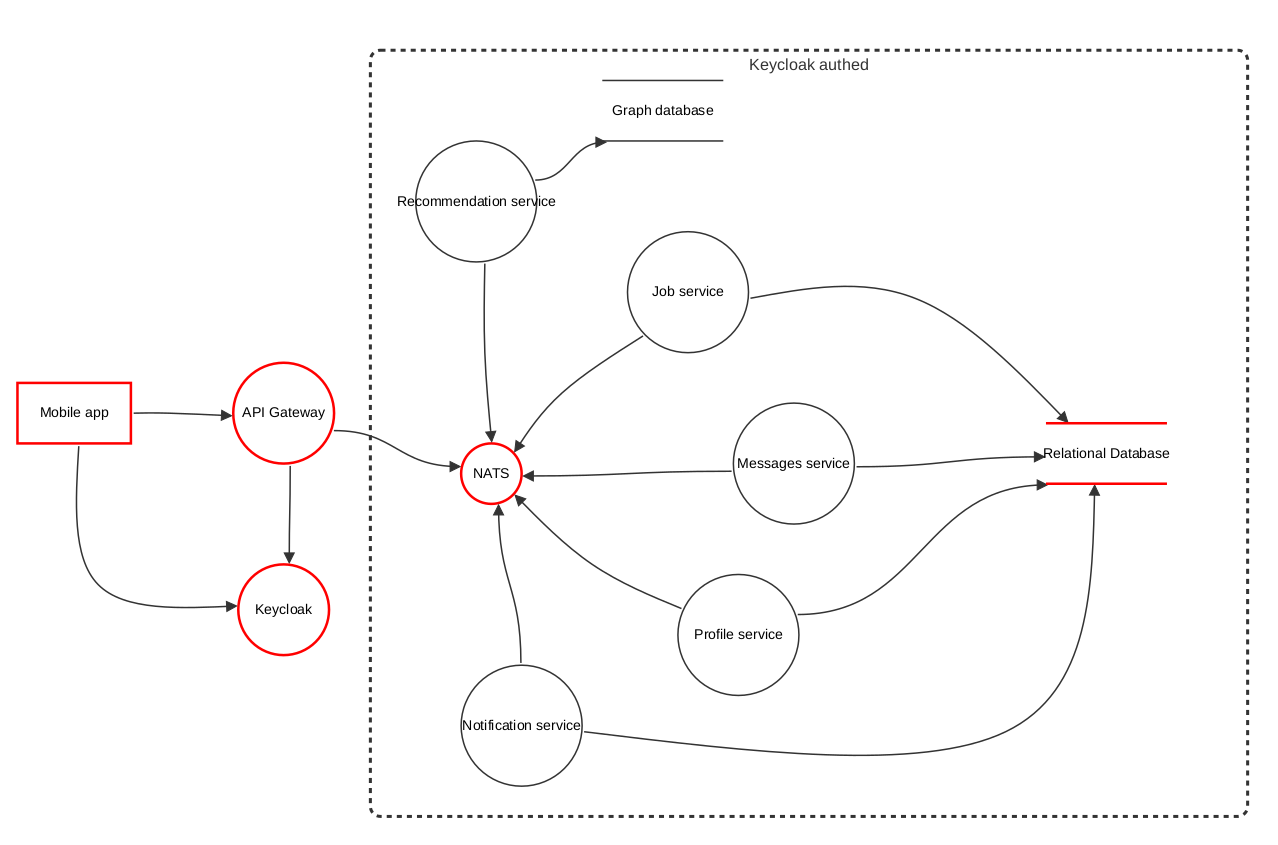
\includegraphics[width=0.8\textwidth]{imgs/threat_dragon.png}
  \caption{Threat dragon infrastructure vulnerabilities diagram}
\end{figure}

\begin{table}[htbp] % Adjusted placement specifier
  \centering
  \small % Smaller font size
  \begin{tabular}{|p{2.5cm}|p{2.5cm}|p{6cm}|p{5cm}|}
  \hline
  \textbf{Target} & \textbf{Threat} & \textbf{Description} & \textbf{Mitigations} \\ 
  \hline
  Mobile app & Man-in-the-middle & A form of cyberattack where an unauthorized third party intercepts and possibly alters communication between two parties without their knowledge or consent. & Since the API uses HTTPS, a man-in-the-middle would only let the attacker get the DNS the user is talking to (if not using a protocol such as DNS over HTTPS) since the HTTPS traffic will be encrypted from end-to-end. \\ 
  \hline
  Backend pods & Elevation of privilege & Elevation of privilege is a security exploit where an attacker gains higher-level access or permissions than originally authorized, typically allowing them to execute actions or access resources beyond their intended scope. & Since the API uses HTTPS, and if the user's machine is not compromised, it is not possible to tamper with the traffic in a useful manner because it is encrypted. \\ 
  \hline
  API Gateway & JWT spoofing & Deceptive practice of forging or altering JSON Web Tokens to impersonate legitimate users or gain unauthorized access to systems and resources. & Our OIDC access token is signed by Keycloak, and the API gateway checks that the signature is correct on the token provided by the user. Therefore, this kind of attack is not possible. \\ 
  \hline
  Relational database & SQL injection & Exploiting SQL vulnerabilities to execute arbitrary SQL code on a database. & Proper input validation and parameterized queries can prevent SQL injection attacks. Regular security audits and updates are also crucial. \\ 
  \hline
  \end{tabular}
  \caption{Description of threats and mitigations}
\end{table}


\bigskip

% Version control
\section{Version control}

% Security features
\subsection{Security features}

We are using GitHub to store our code. We are using the following features of GitHub to
secure our code:

\begin{itemize}
    \item \textbf{Branch protection:} We have protected the main branch of our repository
    to prevent direct pushes to it. This is to prevent someone from pushing code directly
    to the main branch without a review. Moreover, the pull requests are configured to
    only allow merges if the CI pipeline passes and there is at least one approval.
    \item \textbf{Secrets scanning:} We have enabled secrets scanning on our repository.
    This feature scans our code for secrets such as API keys, and alerts us if it finds
    any.
\end{itemize}

\begin{figure}[H]
  \centering
  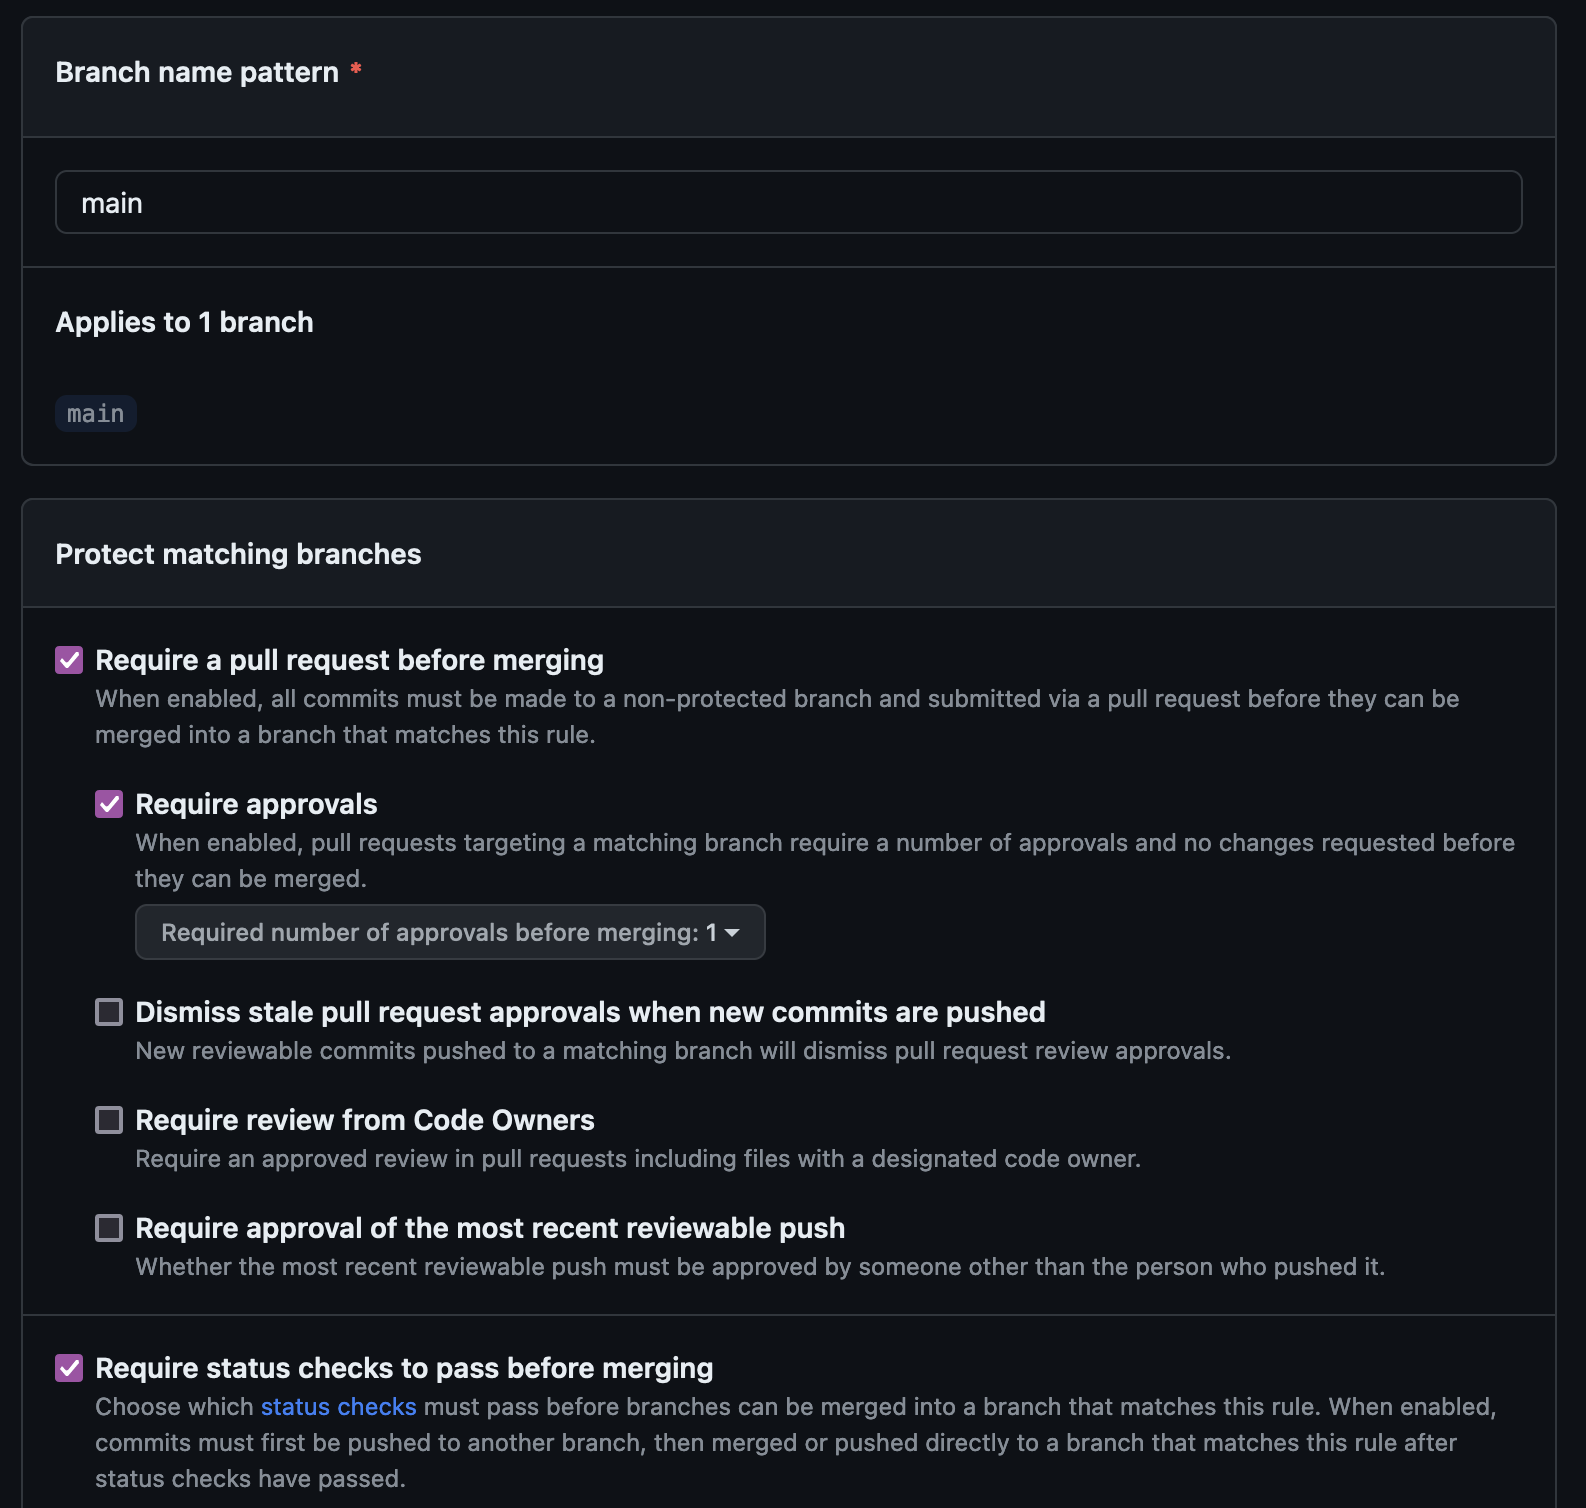
\includegraphics[width=0.8\textwidth]{imgs/branch_protection.png}
  \caption{Branch protection settings}
\end{figure}

\begin{figure}[H]
  \centering
  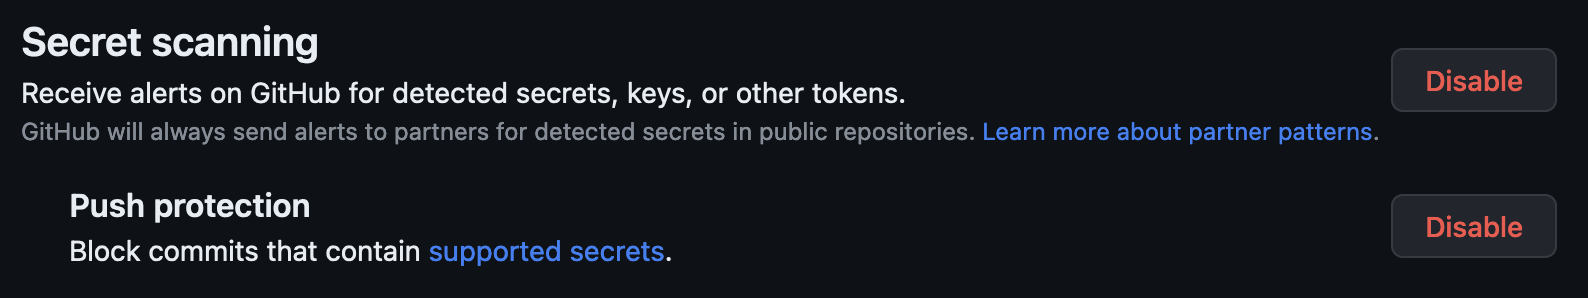
\includegraphics[width=0.8\textwidth]{imgs/secret_scanning.png}
  \caption{Secret scanning status}
\end{figure}

% GitHub Actions
\subsection{GitHub Actions}

We also have GitHub Actions continuous integration pipelines configured to run on every
push and pull requests to the main branch, as well as tags (for the release process).

\medskip
The push and pull request pipeline runs the following steps:

\begin{itemize}
    \item Run the linters for each backend service (ktlint) and the mobile 
    application (ESLint).
    \item Run Snyk to check for vulnerabilities in the code and dependencies for each
    of the backend services (\texttt{snyk/actions/gradle-jdk17}) and the mobile application 
    (\texttt{snyk/actions/node}). The reports of those checks (in the SARIF format) are 
    then uploaded to GitHub CodeQL so they can be seen in the "Security" tab of the repository
    (\texttt{github/codeql-action/upload-sarif}).
    \item Build, sign and push the container images for the backend services (\texttt{docker/build-push-action}).
\end{itemize}

The different CI pipelines can be found \href{https://github.com/thomas-mauran/LinkedOut/tree/main/.github/workflows}{\textbf{here}}.

% Container image signing
\subsection{Container image signing}

Concerning the signature of the container images, we are using a tool called 
\href{https://github.com/sigstore/cosign}{\textbf{cosign}}, which is a tool for signing
OCI images and other artifacts. This tool allows us to sign the container images with 
a private key.

\medskip
In the pipeline, the following actions are used:

\begin{lstlisting}
- name: Install Cosign
uses: sigstore/cosign-installer@v3
[...]
- name: Sign image with Cosign
run: |
    images=""
    for tag in ${TAGS}; do
    images+="${tag}@${DIGEST} "
    done
    cosign sign --yes --key env://COSIGN_PRIVATE_KEY ${images}
env:
    TAGS: ${{ steps.meta.outputs.tags }}
    COSIGN_PRIVATE_KEY: ${{ secrets.COSIGN_PRIVATE_KEY }}
    COSIGN_PASSWORD: ${{ secrets.COSIGN_PASSWORD }}
    DIGEST: ${{ steps.build_and_push.outputs.digest }}
\end{lstlisting}

The first action installs cosign on the runner, and the second action signs the container
image that was previously built and pushed to the container registry. The private key and
password used for signing the image are stored as secrets in the repository.

\medskip
The pipeline containing those actions can be found \href{https://github.com/thomas-mauran/LinkedOut/blob/main/.github/workflows/flow_backend_build_push.yml}{\textbf{here}}.

\medskip
We will see later how those signatures are checked when the container images are deployed
to the Kubernetes cluster.

% Security coding standards
\section{Security coding standards}

During the development of our microservices, we followed some practices to ensure that
our code is secure. Because our microservices are written in Kotlin, and using the
Spring Boot framework, a lot of security features are already built-in or easy to
implement using the framework and its ecosystem.

\medskip
Here are some of the practices we followed:

\begin{itemize}
  \item \textbf{Input validation and output encoding:} For validating user inputs, we
  are using the Spring Boot Validation library to validate the inputs of the API
  endpoints. Kotlin's data classes are used to define the request ("DTOs") and response 
  bodies of the API endpoints, and the validation is done using annotations on those 
  data classes.
  \item \textbf{Auth and password management:} For authentication, we are using the Spring
  Boot Security and OAuth2 Resource Server libraries. Authentication itself is left to Keycloak,
  which is a popular open-source identity provider.
  \item \textbf{Session management:} This is also handled by Keycloak, which provides
  a session management system.
  \item \textbf{Access control:} For this, we are using the Spring Boot OAuth2 Resource
  Server library, which checks the signature of the JWT given by the client against the
  public key of the identity provider (Keycloak).
  \medskip \\
  Once this is verified, we can extract a list of roles from the JWT. Every route needs
  \href{https://github.com/thomas-mauran/LinkedOut/blob/04707ea2f0a31d8f8977ee31a2e7603779aae71f/backend/api_gateway/src/main/kotlin/com/linkedout/backend/config/SecurityConfig.kt#L24}{\textbf{a specific role}} 
  to be accessed. Some routes that are used by administrators are further restricted to
  \href{https://github.com/thomas-mauran/LinkedOut/blob/04707ea2f0a31d8f8977ee31a2e7603779aae71f/backend/api_gateway/src/main/kotlin/com/linkedout/backend/controller/ProfileController.kt#L59}{\textbf{another role}}.
  \item \textbf{Cryptographic practices:} Because we don't directly stored sensitive data in
  this project, we didn't need to encrypt anything. We leave password encryption to Keycloak,
  which is the only entity to know them in the system.
  \item \textbf{Error handling and Logging:} For logging, we are directly printing to the
  standard output and standard error streams, as recommended by the \href{https://12factor.net/logs}{\textbf{twelve-factor methodology}}.
  \item \textbf{Communication security:} Access to the API is done through HTTPS, which is
  managed by the Traefik ingress controller of the Kubernetes cluster. It is configured to
  perform TLS termination and to redirect HTTP requests to HTTPS. The certificate is managed
  by cert-manager, and is issued by Let's Encrypt. You can see a report on the \href{https://www.ssllabs.com/ssltest/analyze.html?d=linkedout.cluster%2d2020%2d5.dopolytech.fr&latest}{\textbf{SSL Labs}} website.
  \item \textbf{Database security:} Each microservice has its own role and logical database
  associated with it in the PostgreSQL database.
  \item \textbf{Memory management:} Because we are using Kotlin on the JVM, we have a 
  garbage collector and the language is modern enough to prevent memory leaks and buffer
  overflows.
\end{itemize}

All the dependencies of the API gateway can be found \href{https://github.com/thomas-mauran/LinkedOut/blob/main/backend/api_gateway/build.gradle.kts}{\textbf{here}}.

\begin{figure}[H]
  \centering
  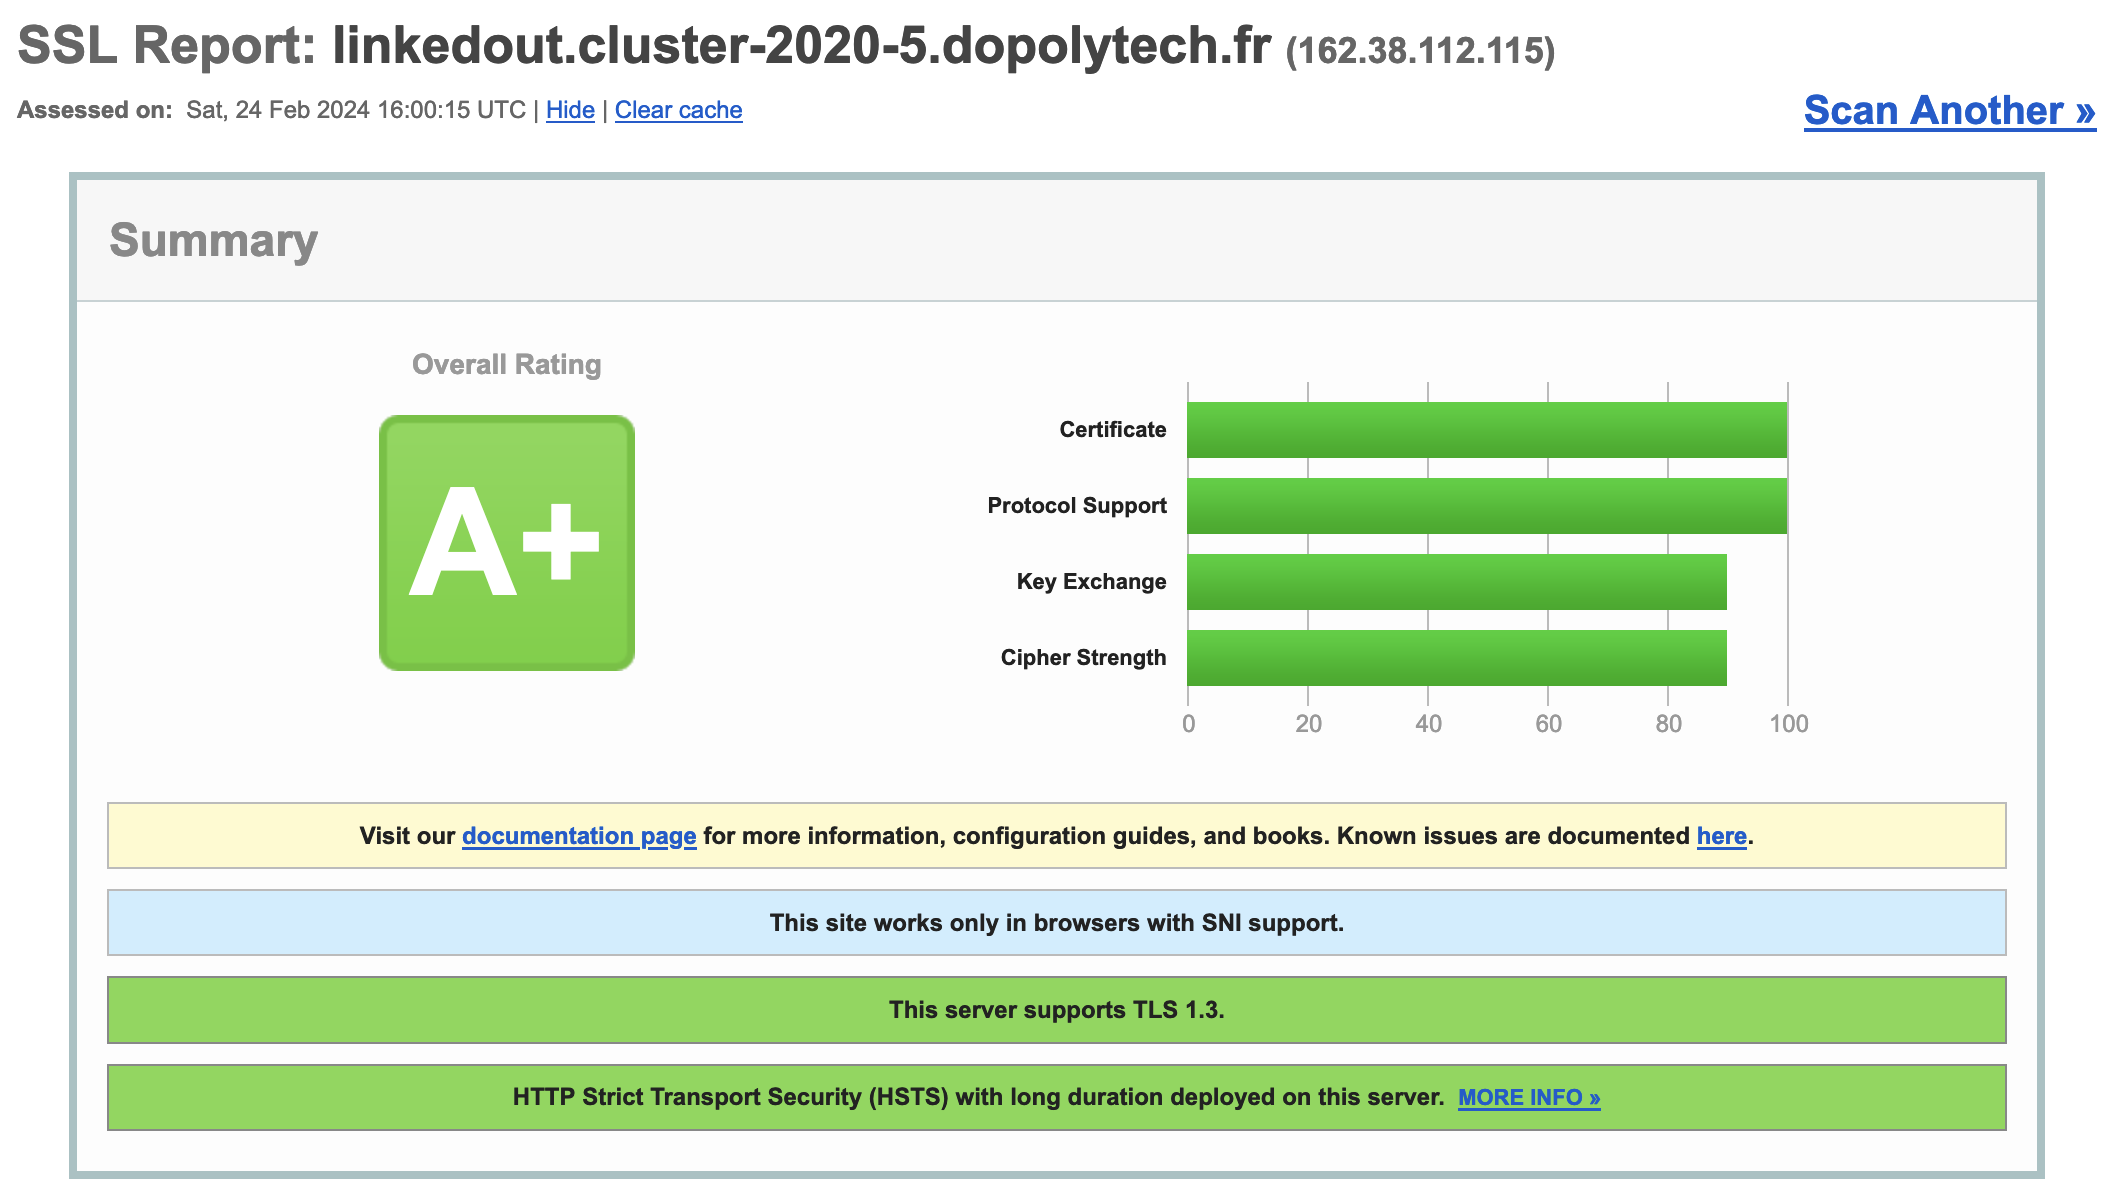
\includegraphics[width=0.8\textwidth]{imgs/ssl_report.png}
  \caption{SSL report of the domain}
\end{figure}

% Securing Docker
\section{Securing Docker}

In the Dockerfile of our microservices, we added directives to create a new user and to
use it when running the container. This is to prevent running the container as root, which
could lead to privilege escalation.

\medskip
The following lines are added to the Dockerfile:

\begin{lstlisting}
RUN addgroup -S linkedout && adduser -S linkedout -G linkedout
[...]
USER linkedout
\end{lstlisting}

This file is available \href{https://github.com/thomas-mauran/LinkedOut/blob/main/backend/Dockerfile}{\textbf{here}}.

% Securing Kubernetes
\section{Securing Kubernetes}

% Container image signature verification
\subsection{Container image signature verification}

After having pushed signed container images to the container registry, we need to verify
the signature of those images before running them on our Kubernetes cluster.

\medskip
To do that, we are using \href{https://kyverno.io/}{\textbf{Kyverno}}, which is a
policy engine for Kubernetes. Once installed on the cluster, we can define policies to
enforce security rules on the resources of the cluster.

\medskip
We have defined a policy that checks the signature of the container images from this
project (so every image that references \texttt{ghcr.io/thomas-mauran/linkedout/*}). The
policy is defined like this:

\begin{lstlisting}
apiVersion: kyverno.io/v1
kind: ClusterPolicy
metadata:
  name: check-linkedout-image-signature
spec:
  validationFailureAction: Enforce
  background: false
  webhookTimeoutSeconds: 30
  failurePolicy: Fail
  rules:
    - name: check-image
      match:
        any:
          - resources: 
              kinds:
                - Pod
      verifyImages:
        - imageReferences:
            - "ghcr.io/thomas-mauran/linkedout/*"
          attestors:
            - count: 1
              entries:
                - keys:
                    publicKeys: |-
                      -----BEGIN PUBLIC KEY-----
                      MFkwEwYHKoZIzj0CAQYIKoZIzj0DAQcDQgAEaFU86MNnoiHTLXkBrgnPO18R5gpo
                      cMic199RKzUa6YftDcDCEovrR0nyzfGp3pKcr4nhjwi3qNRQRHPz76EaWg==
                      -----END PUBLIC KEY-----
\end{lstlisting}

This policy defines the following:

\begin{itemize}
  \item The validation failure action is set to \texttt{Enforce}, which means that the
  policy will deny the creation of resources that do not comply with the policy.
  \item The policy is applied to all resources of kind \texttt{Pod}.
  \item The policy checks the signature of the container whose images are from our
  container registry with the \texttt{ghcr.io/thomas-mauran/linkedout/*} pattern.
  \item The policy checks that the container images are signed with a specific public
  key (the one associated with the private key used to sign the images).
\end{itemize}

This policy is available \href{https://github.com/thomas-mauran/LinkedOut/blob/main/kube/prod/kyverno-policy.yml}{\textbf{here}}.

\begin{figure}[H]
  \centering
  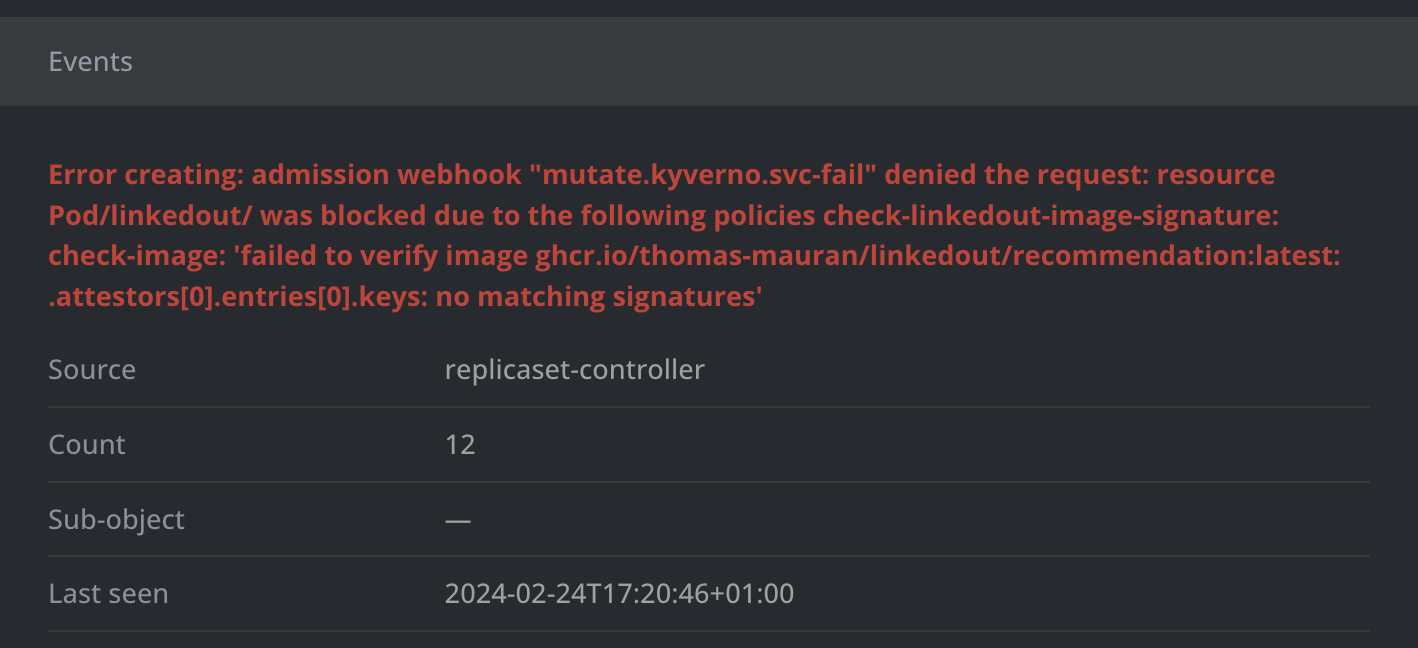
\includegraphics[width=0.8\textwidth]{imgs/kyverno_signature_rejection.png}
  \caption{Kyverno rejecting an unsigned container image}
\end{figure}

% Security context
\subsection{Security context}

Some of the issues that were uncovered by Snyk when we first deployed it were related to
the Kustomize files that we use to deploy our services to the Kubernetes cluster. More
specifically, there was no security context associated with the containers, which means
that the containers were running with more privileges than they needed.

\medskip
We added the following lines to the deployments to restrict the privileges of the containers:

\begin{lstlisting}
[...]
securityContext:
  runAsNonRoot: true
  allowPrivilegeEscalation: false
  readOnlyRootFilesystem: true
  capabilities:
    drop:
      - ALL
\end{lstlisting}

This configuration does the following:

\begin{itemize}
  \item \textbf{runAsNonRoot:} This field specifies that the container must run as a
  non-root user. If the image doesn't specify a user, then the pod will not start.
  \item \textbf{allowPrivilegeEscalation:} This field specifies that the container
  does not allow a process to gain more privileges than its parent process.
  \item \textbf{readOnlyRootFilesystem:} This field specifies that the container's root
  file system is mounted as read-only.
  \item \textbf{capabilities:} This field specifies that the container drops all of its
  capabilities, which are privileged operations that the container can perform.
\end{itemize}

\medskip
An example of a deployment resource can be found \href{https://github.com/thomas-mauran/LinkedOut/blob/main/kube/base/api_gateway/deployment.yml}{\textbf{here}}.

% Resource limits
\subsection{Resource limits}

While not directly related to security, we also added resource limits to the deployments
of our services. This is to prevent a service from using too many resources and potentially
crashing a node, creating a denial of service.

\medskip
While running, each service of the backend uses around 300MiB of memory and 400m of CPU. However,
when starting, they are using a lot more resources for a short period of time. Knowing that,
and taking into account the capacity of the cluster, we decided to set the following limits:

\begin{lstlisting}
[...]
  resources:
    requests:
      memory: "1Gi"
      cpu: "0.5"
    limits:
      memory: "2Gi"
      cpu: "1"
\end{lstlisting}

This configuration does the following:

\begin{itemize}
  \item \textbf{Memory request:} This field specifies that the container requests 1GiB of
  memory.
  \item \textbf{CPU request:} This field specifies that the container requests 0.5 of a CPU.
  \item \textbf{Memory limit:} This field specifies that the container is limited to 2GiB of
  memory.
  \item \textbf{CPU limit:} This field specifies that the container is limited to 1 of a CPU.
\end{itemize}

The configured limits are available \href{https://github.com/thomas-mauran/LinkedOut/blob/main/kube/prod/add-resource-limits.patch.yml}{\textbf{here}}.

% Network policies
\subsection{Network policies}

Network policies are a kind of resources in Kubernetes that allow you to define how groups
of pods are allowed to communicate with each other and other network endpoints. Configuring
them correctly can help to prevent unauthorized access to the services running in the cluster
by simply denying all traffic by default and only allowing the necessary, expected traffic.

\medskip
By looking at the threat model that we previously defined, we can infer some rules that
we can apply on the cluster.

\medskip
On the ingress side:

\begin{itemize}
  \item The microservices don't need to accept any incoming traffic.
\end{itemize}

On the egress side:

\begin{itemize}
  \item The microservices need to be able to communicate with the NATS message broker.
  \item The microservices need to be able to communicate with the PostgreSQL database.
  \item The microservices need to be able to communicate with the Neo4j database.
  \item The microservices need to be able to communicate with the Minio object storage server.
\end{itemize}

This leads to the following network policy for the microservices:

\begin{lstlisting}
apiVersion: networking.k8s.io/v1
kind: NetworkPolicy
metadata:
  name: microservices
spec:
  podSelector:
    matchLabels:
      network-group: microservices
  policyTypes:
    - Ingress
    - Egress
  egress:
    - to:
      - podSelector:
          matchLabels:
            app.kubernetes.io/name: nats
      - podSelector:
          matchLabels:
            app.kubernetes.io/name: postgresql
      - podSelector:
          matchLabels:
            helm.neo4j.com/neo4j.name: linkedout
      - podSelector:
          matchLabels:
            app.kubernetes.io/name: minio  
\end{lstlisting}

\textbf{Note:} While not shown here, we also add to add a second network policy to allow
the pods to communicate with the in-cluster DNS server.

\medskip
The network policies are available \href{https://github.com/thomas-mauran/LinkedOut/blob/main/kube/prod/network-policies.yml}{\textbf{here}}.

\end{document}
